\newpage
\section{Obfuscation Techniques} \label{sec:anti_reverse_engineering}
\begin{framed}
	\begin{definition} 
		\underline{Obfuscation} is the action of making something obscure, unclear, or unintelligible.
		\begin{flushright}
			\hfill{}{Oxford Dictionaries~\cite{od:obfuscation}}
		\end{flushright}
	\end{definition}
\end{framed}

\paragraph{}
Reverse engineering is a inherently complicated process for it requires the reverse engineer to think backward to rediscover buried knowledge, know-how and details from artefacts. This process can be made further more complicated by the artefacts' engineers through the use of obfuscation, a family of techniques that belongs to the anti reverse engineering techniques. The family of obfuscation techniques provides means to make programs more opaque to scrutiny by transforming them into new programs that have the same computational effect while being harder to analyse~\cite{Dang:2014:PRE:2636663}. Anti reverse engineering is a broader family for it also contains techniques that aim, for example, at thwarting reverse engineering tools, detecting virtual machines, and so on.

\paragraph{}
When obfuscation is applied to programs, a harsh reality has to be understood. There is no such thing as a protection which provides a fully opaque filter. Programs are usually being shipped in executables files that are understandable either by the hardware or specific software, and in order to provide a specific behaviour, these executables have to lay a detailed description of that behaviour. One could make the comparison with a blueprint of any kind of engineered artefact. Making it hard to read won't prevent someone motivated enough to make sense out of it, but it can wear some reverse engineers out by making them give up and moving on if the process is slow and painful enough. Not any problem has a neat solution, and preventing reverse engineering is one of these problems. As hinted above, security through obscurity, a solution that is widely discouraged, is the only alternative that can mitigate the risks of having a program being reverse engineered.

\paragraph{}
According to the book \textit{Practical Reverse Engineering: x86, x64, ARM, Windows Kernel, Reversing Tools, and Obfuscation}~\cite{Dang:2014:PRE:2636663}, the obfuscation techniques can be sorted into two categories: Data-based obfuscation and control-based obfuscation. Individually, they do not provide much obscurity. It is only when they are applied together that the reverse engineering process becomes more challenging. The analogy made by Jakubowski et al~\cite{jakubowski2009iterated} about round based cryptography and the iterative application of obfuscation techniques illustrates very well this idea: “A cryptographic algorithm's round is made of basic arithmetic operations (addition, exclusive or, etc.) that perform trivial transformations on the inputs. Considered individually, a round is weak and prone to multiple forms of attacks. Nevertheless, applying a set of rounds multiple times can result in a somewhat secure algorithm. That is the objective of an obfuscator. The objective of the attacker is to discern the rounds from the global obfuscated form and to attack them at their weakest points.”. The remaining of this section will be dedicated to describe known obfuscating techniques that could make the rounds of a practical obfuscator.

\subsection{Data-based Obfuscation}
\subsubsection{Constant Unfolding}
\paragraph{}
Constant folding is a compiler optimisation technique that consists of evaluating constant expressions at compile time and replace the constant expressions by their values~\cite{aho1986compilers}. When writing an expression such as $tau = 3.14 * 2$, one can easily see that reducing it at compile time into $tau = 6.28$ will not alter the semantic of the original program while increasing the runtime performance.

\paragraph{}
Applying constant unfolding at the assembly level is not always as straight forward as it could be in a higher level programming language. For example, in the situation where we want to unfold an expression that sets the content of the $ax$ register to $0x200$, we could use the following expression: \\

\begin{lstlisting}[caption={Example of constant folding.}, label={lst:constant_unfolding}, frame=tlrb, language={[x86masm]Assembler}, otherkeywords={.CODE}]
mov ax, 100h
mov bx, 100h
add ax, bx
\end{lstlisting}

Compared to the folded expression, this one will not only change the content of the $bx$ register, but also the content of the $eflags$ register. More precisely, it will change the content of the overflow flag, the sign flag, the zero flag, the adjust flag, the carry flag, and the parity flag~\cite{guide2011intel}. One has thus to be careful when applying constant unfolding in the context of an assembly language that has side effects for they can change the semantic of the program. 

\paragraph{}
Countering this technique is pretty straight forward, so applying the constant folding optimisation will reduce the expressions to constants.

\subsubsection{Data-Encoding Schemes}
\paragraph{}
One could encode the values of a program stored in the variables and the constants while adding an encoding and decoding function to allow to manipulate them during run time. A simple example would be to have an encoding function that adds the value $x$ and a decoding function that subtracts the same value $x$ of its argument. The major flaws of this technique are that the encoding and decoding functions have to be inside the program, that the variables and constants have to be decoded and thus exposed when used, and lastly that a constant folding optimisation would discard it. 

\begin{framed}
	\begin{definition} 
		A \underline{homomorphism} is an operation-preserving mapping between two algebraic structures.
		\begin{flushright}
			\hfill{}{Oxford Dictionaries~\cite{od:obfuscation}}
		\end{flushright}
	\end{definition}
\end{framed}

\paragraph{}
Homomorphism could be a better solution for it does not make decoding variables mandatory to manipulate them and so it does not expose them. Homomorphism is an operation-preserving mapping between two algebraic structures. To better illustrate this concept, let's take two groups, $A$ and $B$, and two operations, $+_A$ and $+_B$, belonging to the group mentioned in the subscript. The function $f$ is an homomorphism between the sets belonging to $A$ and $B$ if $f(x+_Ay) = f(x)+_Bf(y)$. It is said that this notion can be generalised to arbitrary algebraic structures such as rings and, for example, the addition and multiplication operators. For more information on this topic, see the work of Zhu and Thomborson~\cite{zhu2005provable}.

\subsubsection{Dead Code Insertion}

\paragraph{}
Dead code is the name given to instructions whose results do not affect the behaviour of the program~\cite{debray2000compiler}. They could either never be executed, or have no effect in the current computation. Since they only make the executable files bigger in size, most compilers will always try to eliminate the high level instructions which result in dead code once compiled. This method is called dead code elimination. See \textit{Advanced Compiler Design and Implementation}~\cite{steven1997advanced} for more information on the topic.

\paragraph{}
Dead code insertion is the exact opposite of what has been explained above. One can insert instructions that either do not alter the behaviour of the code or are applied to dead registers\footnote{A dead register is a register which is not used.}. The main goal of this technique is to make the code harder to read, forcing the reverser to decide whether an instruction is meaningful or not.

\paragraph{}
An example of dead code insertion is illustrated in Listing~\ref{lst:dead_code_insertion}. The semantic of the function is to sum the two parameters that it is applied to. While the two last lines are necessary to provide the desired outcome, all that comes before is not. The variable $w$ is never used, and the conditional branch will never be taken. If compiled with the dead code elimination optimisation activated, they would not make it to the machine code.\\

\begin{lstlisting}[caption={Example of function with dead code.}, label={lst:dead_code_insertion}, frame=tlrb, language={c++}]
int add(int x, int y) {
	int w = 50;
	if(false) {
		printf("dead code");
	}
	int result = x + y;
	return result;
}
\end{lstlisting}

\paragraph{}
In the example, the variable $w$ is said to be dead for it has no effect on the computation. On the other hand, the variable result is said to be live since it carries the result of the addition. The same idea can be applied to registers, some partake in the computation, some others don't. This notion is important because when an obfuscator adds dead assembly code into a program, it might have to avoid using live registers to prevent altering the semantic of the program.

\subsubsection{Arithmetic Substitution via Identities} \label{sec:arithmetic_substitution_via_identities}
\paragraph{}
When dealing with mathematics, there usually are plenty of different ways to solve a single problem. Some are easier to understand than others, and as expected when trying to obfuscate programs, the harder the better. Arithmetic substitution is about substituting mathematical expressions with semantically equivalent but syntactically different expressions using identities. One of such identities is the following: Instead of simply adding $1$ to a register when needed, one could write an expression that $xor$ the value of a register with $0XFFFFFFFF$ and apply the unary minus operator to the result. For the binary value $0011$ ($3$), xoring it with itself gives $1100$ and negating the result yields $0100$ ($4$). To be noted that this substitution only works in a system using the two's complement signed number representation.

\paragraph{}
Below are listed a few identities from the book \textit{Practical Reverse Engineering: x86, x64, ARM, Windows Kernel, Reversing Tools, and Obfuscation}~\cite{Dang:2014:PRE:2636663}. The symbol $\sim$ is the not operator, $rotate\_\{left, right\}(x, y)$ performs a rotation of $y$ bits on $x$ in the chosen direction, $nb\_bits(x)$ returns the number of bits that makes a value $x$.
\begin{itemize}
	\item $-x = \sim x + 1$
	\item $x + 1 = - \sim x$
	\item $x-1 = \sim - x$
	\item $rotate\_left(x, y) = (x << y)\ |\ (x >> (nb\_bits(x)-y))$
	\item $rotate\_right(x, y) = (x >> y)\ |\ (x << (nb\_bits(x)-y))$
\end{itemize}

\paragraph{}
The Information Security Group of the University of Applied Sciences and Arts Western Switzerland has developed an obfuscator for the LLVM\footnote{LLVM is a collection of modular and reusable compiler tool chain technologies. See \url{http://llvm.org/} for more information.} Intermediate Representation, or IR for short, language~\cite{ollvm} that uses different substitutions such as the following:
\begin{itemize}
	\item $b$ \& $c$ becomes $(b\ \oplus \sim c)$ \& $b$
	\item $b\ |\ c$ becomes $(b$ \& $c)\ |\ (b \oplus c)$
	\item $a \oplus b$ becomes $(\sim a$ \& $b)\ |\ (a$ \& $ \sim b)$
	\item $a = b + c$ becomes $r = rand (); a = b - r; a = a + b; a = a + r$
\end{itemize} 

\paragraph{}
Just like using a single obfuscation technique to harden your program is not very useful, applying only one identity will yield poor results. One will instead want to apply many of them, possibly on the result of other permutations. Creativity and the overhead gained from expanding simple operations into more complex ones are the only limitations of this obfuscation technique. Combining the substitution will make it harder for a reverser to understand the underlying logic but will have an impact on the overall performance and size of the program.

\subsubsection{Pattern-Based Obfuscation} \label{sec:pattern_based_obfuscation}
\paragraph{}
Pattern-Based Obfuscation is, in a way, similar to the arithmetic substitution presented in Section~\ref{sec:arithmetic_substitution_via_identities}. Instead of substituting mathematical operations, this technique consists of substituting a set of adjacent instructions into another set of instructions that has an equivalent semantic. One example can be observed in Listing~\ref{lst:jmp_push_ret_1} and Listing~\ref{lst:jmp_push_ret_2}, where the $jump$ instruction is said to be equivalent to pushing the destination address on the stack and calling the $ret$ instruction right after. Because the semantic of $ret$ is to $pop$ the first at the top of the stack and $jump$ to that value, the semantic of $jmp$ is replicated. \\ \\

\noindent\begin{minipage}{.45\textwidth}
	\begin{lstlisting}[caption={Program equivalent to the one in Listing~\ref{lst:jmp_push_ret_2}. Semantic equivalence preserved.}, label={lst:jmp_push_ret_1}, frame=tlrb, language={[x86masm]Assembler}, otherkeywords={.CODE}]
jmp addr
	\end{lstlisting}
\end{minipage}\hfill
\begin{minipage}{.45\textwidth}
	\begin{lstlisting}[caption={Program equivalent to the one in Listing~\ref{lst:jmp_push_ret_1}. Semantic equivalence preserved.}, label={lst:jmp_push_ret_2}, frame=tlrb, language={[x86masm]Assembler}]
push addr
ret
	\end{lstlisting}
\end{minipage}

\paragraph{}
Other examples could include the $push$ and $pop$ operations, which take or put a value on the stack and increase or decrease the value of the stack pointer. Listing~\ref{lst:push_mov_sub_1} and Listing~\ref{lst:push_mov_sub_2} show the former identity, Listing~\ref{lst:pop_mov_add_1} and Listing~\ref{lst:pop_mov_add_2} show the later identity.\\ \\

\noindent\begin{minipage}{.45\textwidth}
	\begin{lstlisting}[caption={Program equivalent to the one in Listing~\ref{lst:push_mov_sub_2}. Semantic equivalence preserved.}, label={lst:push_mov_sub_1}, frame=tlrb, language={[x86masm]Assembler}, otherkeywords={.CODE}]
push eax
	\end{lstlisting}
\end{minipage}\hfill
\begin{minipage}{.45\textwidth}
	\begin{lstlisting}[caption={Program equivalent to the one in Listing~\ref{lst:push_mov_sub_1}. Semantic equivalence preserved.}, label={lst:push_mov_sub_2}, frame=tlrb, language={[x86masm]Assembler}]
mov dword ptr [esp], eax
sub esp, 4
	\end{lstlisting}
\end{minipage}

\noindent\begin{minipage}{.45\textwidth}
	\begin{lstlisting}[caption={Program equivalent to the one in Listing~\ref{lst:pop_mov_add_2}. Semantic equivalence preserved.}, label={lst:pop_mov_add_1}, frame=tlrb, language={[x86masm]Assembler}, otherkeywords={.CODE}]
pop eax
	\end{lstlisting}
\end{minipage}\hfill
\begin{minipage}{.45\textwidth}
	\begin{lstlisting}[caption={Program equivalent to the one in Listing~\ref{lst:pop_mov_add_1}. Semantic equivalence preserved.}, label={lst:pop_mov_add_2}, frame=tlrb, language={[x86masm]Assembler}]
mov dword ptr [eax], esp
add esp, 4
	\end{lstlisting}
\end{minipage}

\paragraph{}
It is once again important to note the side effects an instruction can have when using it as a substitution. In the first example, where the $jump$ instruction is replaced by a $push$ and $ret$, no flags are affected and so they are both semantically equivalent. On the other hand, the $push$ and $pop$ equivalents are not semantically equivalent for $add$ and $sub$ change flags.

\subsection{Control-based Obfuscation}
\subsubsection{Inline and Outline Expansion}
\paragraph{}
Inline expansion is a compiler optimisation which consist of replacing specific function invocations by their body, which are altered beforehand to take into account the new way the parameters and the return value will be passed~\cite{aho1986compilers}. One advantage of this technique is that it makes the code faster by removing all the machinery that is necessary when calling a function. The main disadvantage is that the code will grow in size since the body will be duplicated as many times as it is called.

\paragraph{}
Outline expansion is simply the opposite operation, it consists of extracting a piece of code, turning it into a function, and adding a function call for that function. The advantage and inconvenient of using this technique are obviously the opposite of the ones for inline expansion.

\paragraph{}
Using inline and outline expansion the right way can greatly degenerate the call graph of the application. A call graph is simply a graph which shows what functions a function might be calling. A simple example can be observed in Figure~\ref{fig:call_graph}. By doing so, the graph will be greatly harder to read, and so to reason about.

\begin{figure}[!htb]
	\centering
	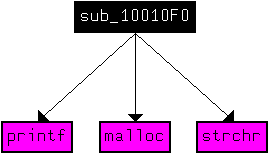
\includegraphics[width=0.5\textwidth]{reverse_engineering/call_graph.png}
	\caption{Part of the call graph of the Microsoft Resource Compiler generated with IDA pro.}
	\label{fig:call_graph}
\end{figure}

\subsubsection{Removing Sequential and Temporal Locality}
\paragraph{}
A basic block of code is a sequential listing of code which does not have any “in-branches” other than its entry point and no “out-branches” except its exit point. When a compiler encounters such a block, it will generate one continuous block of instructions. This property, called sequential locality, makes reverse engineering easier for one can simply read the instructions of a block in a sequential order, without caring about branches, to get a gist of its purpose.

\paragraph{}
Compilers will also put temporally related blocks next to each other. For example, if the exit point of a block is the entry point of another block, they will be stored side by side in the executable file. This property is called the sequential locality of temporally related code~\cite{Dang:2014:PRE:2636663}. These two properties are important for a performance point of view because of how CPU caching is done, that is by decoding the next logical instructions in advance in hope that they will indeed be part of the execution path. 

\paragraph{}
This technique, as its name suggests, consists of modifying the machine code so that these two properties are not satisfied anymore. By inserting unconditional branches inside the blocks of code and displacing the temporally related block, a reverse engineer will have a harder time reasoning about the code. This technique will not be of any use against automated deobfuscation tool.

\pagebreak

\subsubsection{Opaque Predicates} \label{sec:opaque_predicates}
\begin{framed}
	\begin{definition}
		A predicate P is \underline{opaque} if a deobfuscator can deduce its outcome only with great difficulty, while this outcome is well known to the obfuscator.
		\begin{flushright}
			\hfill{}{A taxonomy of obfuscating transformations~\cite{collberg1997taxonomy}}
		\end{flushright}
	\end{definition}
\end{framed}

\paragraph{}
The idea behind opaque predicates (boolean expressions) is that, whether they will be evaluated to true of false will not clear from the point of view of an attacker until being evaluated, while always evaluating to the same value. One usage is to use such a predicate in a conditional branch, turning it into an unconditional branch. Of course, that is information a disassembler will not have since it will not reduce the expression. As a result, another, dead, branch will be added into the control flow graph of the application. From there, one could either put junk code or keep complexing the control flow graph by adding branches.

\paragraph{}
A simple example of opaque predicate would be comparing two different constant numbers and using the jump not equal instruction to branch to the valid continuation of the program. Another, more complex, example could be made by using the greatest common divisor (GCD) algorithm. Being an associative binary operator, one could choose a set of integers and recursively pick and apply numbers to the result of the previous application of the GCD algorithm. When the set gets fully consumed, checking the parity of the result will give a true or false answer. Pseudo code for this algorithm can be found in Listing~\ref{lst:gcd_algorithm}. \\

\begin{lstlisting}[caption={Pseudo code for an opaque predicate based on the greatest common divisor algorithm.}, label={lst:gcd_algorithm}, frame=tlrb]
let s := {...}
let accumulator := random_get(s)

while s != empty
accumulator := gcd(accumulator, random_get(s))
end while

if (accumulator % 2 == 0) 
...
then
...
end if
\end{lstlisting}

\paragraph{}
In \textit{Practical Reverse Engineering}~\cite{Dang:2014:PRE:2636663} is proposed a variant that works as follows: Instead of having an opaque predicate that always evaluates to the same value, one could make it evaluate randomly to true or false while having the two branches being semantically equivalent. As they would pass the control flow to the same instruction once finished, it would give rise to a diamond shaped control flow graph.

\paragraph{}
For more information on the topic, one might be interested in reading these two articles: \textit{Manufacturing cheap, resilient, and stealthy opaque constructs}~\cite{collberg1998manufacturing} and \textit{A Taxonomy of Obfuscating Transformations}~\cite{collberg1997taxonomy}.

\subsubsection{Interleaving Function's Body}
\paragraph{}
As its name suggests, this technique consists of taking functions' body and splitting them into fragments that are then interleaved and connected with unconditional jumps composed with opaque expressions. These expressions will have to reduce to the memory addresses of the next fragment. That way, it is not obvious which fragments belong to which functions. This technique will make it harder, both for a reverse engineer and a tool, to make sense of the code. An example where two functions are interleaved can be observed in Listing~\ref{lst:interleaving_2}. \\ \\

\noindent\begin{minipage}{.45\textwidth}
	\begin{lstlisting}[caption={Two functions and their body.}, label={lst:interleaving_1}, frame=tlrb, language=C]
function_1() {
	function_1_step_1
	function_1_step_2
	function_1_step_3
}
	
function_2() {
	function_2_step_1
	function_2_step_2
	function_2_step_3
}
	\end{lstlisting}
\end{minipage}\hfill
\begin{minipage}{.45\textwidth}
	\begin{lstlisting}[caption={Interleaving of the two functions found in Listing~\ref{lst:interleaving_2}. Inspired from the book Reversing: \textit{Reversing: Secrets of Reverse Engineering}~\cite{eilam2005reversing}.}, label={lst:interleaving_2}, frame=tlrb, language={[x86masm]Assembler}]
function_2_step_1
	jmp opaque_expression
function_1_step_3
	ret
function_1_step_1
	jmp opaque_expression
function_2_step_2
	jmp opaque_expression
function_2_step_3   
	ret     
function_1_step_2
	jmp opaque_expression
	\end{lstlisting}
\end{minipage}

\subsubsection{Processor Based Control Indirection}
\paragraph{}
This technique consists of obfuscating the two most obvious ways branching is done in machine code, that is with the $call$ and the $jmp$ instructions. The interest is that, besides the fact that the listing produced by a disassembler will be harder to understand for humans, many tools will not recognise the potential branching, and so won't be able to provide as many details as they usually would. 

\paragraph{}
Whenever a disassembler discovers a $call$ instruction, it will interpret the address applied to the instruction as the entry point of a function. Since functions are made to give back the control once finished, the disassembler will also assume the presence of the $ret$ instruction, signalling the end of the function. Replacing these two instructions by semantically equivalent sequences of instructions will then, for example, prevent the generation of the control flow graph.

\paragraph{}
In Listing~\ref{lst:masm_processor_based_control_indirection} can be seen an example where $call$ has been replaced by three instructions: One to get the instruction pointer ($ip$), one to increment the $ip$ value to point toward after the function call, and finally a jump to the $foo$ function. When loaded into IDA Pro, the $foo$ function will not appear in the call graph nor in the control flow graph. \\

\begin{lstlisting}[caption={MASM code which hides the function call to $foo$ by using a set of instructions with an equivalent effect.}, label={lst:masm_processor_based_control_indirection}, frame=tlrb, language={[x86masm]Assembler}]
getEip PROC
	mov eax, [esp]
	ret
getEip ENDP

foo PROC
	invoke MessageBox, NULL, addr MsgBoxText, 
	addr MsgBoxCaption, MB_OK
	ret
foo ENDP

start:
	call getEip		; This
	add eax, 06h	; is
	push eax		; replacing
	jmp foo			; call foo
	...				; getEip + 06h
end start
\end{lstlisting}

\paragraph{}
For the $jmp$ instruction, it is fairly easy to emulate it with a $push$ and $ret$ as explained in Section~\ref{sec:pattern_based_obfuscation}. It is also feasible to use $call$ on the landing address and poping the return address that will have been pushed by the $call$ instruction. By doing so, the control flow graph will get polluted.

\subsection{Combining Data and Control Flow Techniques}
\subsubsection{Junk Code Insertion}
\paragraph{}
This technique presented in the book \textit{Practical Reverse Engineering}~\cite{Dang:2014:PRE:2636663} uses the dead code insertion technique and the opaque predicate technique to try to thwart the disassembler by making it follow specifically crafted branches that will not be followed by a CPU. The branch can contain simple dead code or jumps to invalid addresses, which would make the disassembler desynchronize.

\paragraph{}
A simple example written in MASM can be observed in Listing~\ref{lst:junk_code_insertion}. In the situation where eax starts with the value zero, adding it to itself will never cause overflow. As a consequence, the conditional jump will always be taken, skipping the junk code. The disassembler, not being aware of this, will think that this function is recursively calling itself and that the $ret$ instruction is part of another function. When loaded in IDA Pro, the control flow graph in Figure~\ref{fig:control_flow_graph_junk_code} appears. \\
\begin{lstlisting}[caption={Inserting junk code to trick the disassembler into believing that the function is recursive and that $ret$ is part of another function.}, label={lst:junk_code_insertion}, frame=tlrb, language={[x86masm]Assembler}]
start:
	add eax, eax
	jno end_junk
	jmp start
	ret
end_junk:
	invoke ExitProcess, NULL
end start
\end{lstlisting}


\begin{figure}[!htb]
	\centering
	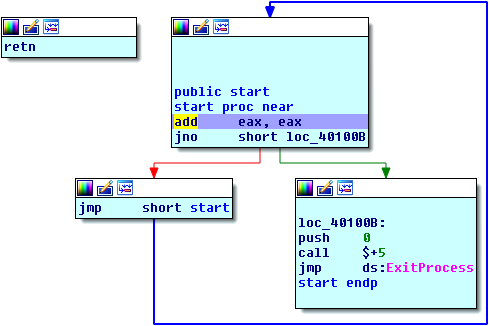
\includegraphics[width=0.7\textwidth]{reverse_engineering/control_flow_graph_code_junk.png}
	\caption{Part of the call graph of the Microsoft Resource Compiler.}
	\label{fig:control_flow_graph_junk_code}
\end{figure}

\subsubsection{Control Flow Graph Flattening}
\paragraph{}
Control flow graph flattening is a technique which consists of transforming a source code into another source code that will produce a flattened CFG once statically analysed. A flattened CFG is a graph which has one dispatcher node that is connecting every other nodes, and every other nodes are connected to the dispatcher node to give it back the control flow once over.  A reverse engineer, when faced with a flattened CFG, will not be able to follow the branches easily, making it harder to perform static analysis. On the other hand, the extra branching will have a cost on the overall performance of the application.

\paragraph{}
Below is given a simplified algorithm for CFG flattening. It has been proposed in the article titled \textit{Obfuscating C++ Programs via Control Flow Flattening}~\cite{laszlo2009obfuscating}.
\begin{enumerate}
	\item Break a function's body into basic blocks and put them next to the other. Note that before this operation, the blocks were not at the same level of nesting.
	\item Encapsulate the blocks in a switch-like construct, where each block has its own case/break separator.
	\item Wrap the whole construct in a loop.
	\item Add a state variable that gets updated at the end of every basic block. This variable is used by the construct to find the next basic block to be executed.
\end{enumerate}

\paragraph{}
An example of CFG flattening can be observed in Figure~\ref{fig:control_flow_graph_flattening}, which is the result of applying the algorithm on the code found in Listing~\ref{lst:control_flow_graph_flattening}. One should pay attention to how the while loop from the original code has been rewritten into two basic blocks: One for the body and one to check whether the predicate still holds or not.

\pagebreak

\begin{lstlisting}[caption={Simple code to compute the factorial of 50.}, label={lst:control_flow_graph_flattening}, frame=tlrb, language=C]
int main(int argc, char** argv) {
	int n = 50;
	int r = 1;
	while (n != 0) {
		r = r * n;
		n = n - 1;
	}
}
\end{lstlisting}

\begin{figure}[!htb]
	\centering
	\includegraphics[width=0.7\textwidth]{reverse_engineering/cfg_flattening.png}
	\caption{Control flow graph of the code from Listing~\ref{lst:control_flow_graph_flattening} once flattened. Example inspired from \textit{Obfuscating C++ Programs via Control Flow Flattening}~\cite{laszlo2009obfuscating}.}
	\label{fig:control_flow_graph_flattening}
\end{figure}


\subsubsection{Virtual Machines}
\paragraph{}
It has been said before that some languages are first compiled into an intermediate representation (IR) to provide, amongst other things, better portability. Whenever a file containing such code needs to be executed, a just-in-time (JIT) compiler will dynamically compile the intermediate instructions into machine code and let the CPU execute them. 

\paragraph{}
For a reverse engineer to analyse such language, he or she needs to know the semantic of the instructions composing the language combined with the architecture of the virtual machine over which the instructions are being interpreted. For well known IRs such as the Java Bytecode, one can simply refer to the official documentation, but when both the language and the architecture are kept secret, the analysis suddenly turns into a tedious task. 

\paragraph{}
Contrary to mainstream uses of virtual machines, obfuscating virtual machines will embed the JIT compiler (or interpreter) inside the executable file, next to the intermediate instructions. The interpreter can obviously not be written using the IR for the CPU would not be able to make sense out of it. Whenever such executable is launched, the control flow is given to the interpreter which will proceed to read and evaluate the intermediate instructions. As a result, the interpreter is the only part of code that can be statically analysed.

\paragraph{}
The disadvantages of this method are that it is very complicated to engineer a virtual machine, and the performance of the application will be greatly diminished.

\subsection{Other Anti Reverse Obfuscation}
\paragraph{}
As explained previously, it is a tedious process to preserve the semantical equivalence when tinkering with assembly code. Moreover, obfuscating a program has a cost that one might not be keen to pay, or simply cannot afford. The techniques presented in the remaining of this section also aim at slowing down the reverse engineering process, but in a way that does not require rewriting code. They thus do not fall into the obfuscating family any more but are worth being acknowledged nonetheless. To be noted that, once again, using only one technique will not produce a good protection. As the national motto of Belgium says, “unity makes strength”.    

\subsubsection{Removing Symbolic Information}
\paragraph{}
Symbolic information are pieces of information that can be found in binary files such as executables and dynamic-link libraries (DLLs). According to their nature, they can help a reverse engineer carrying out his or her task with very little effort and so must be taken into consideration. The amount of information found in a file varies according to its type and the compiler used to produce the file. The two most verbose cases are the import/export tables and when dealing with partially compiled code such as Java bytecode.

\paragraph{}
An executable using the PE format presented in Section~\ref{sec:executable_file_format} will contain an Import Address Table (IAT). In it, it could be found the name of the modules that contain functions needed by the executable, as well as the name of the functions or their ordinal inside the module. Names and ordinals are equivalent for they uniquely identify one function, but they differ on how they identify it. The name is a textual representation while the ordinal is just a number. It is obvious that more can be inferred from a name since they are usually chosen to describe their behaviour. In Figure~\ref{fig:import_table} can be observed the import table of a program that checks if a debugger has been attached to it. It would not have been as obvious if “isDebuggerPresent” had been replaced by, let's say, “6”.

\begin{figure}[!htb]
	\centering
	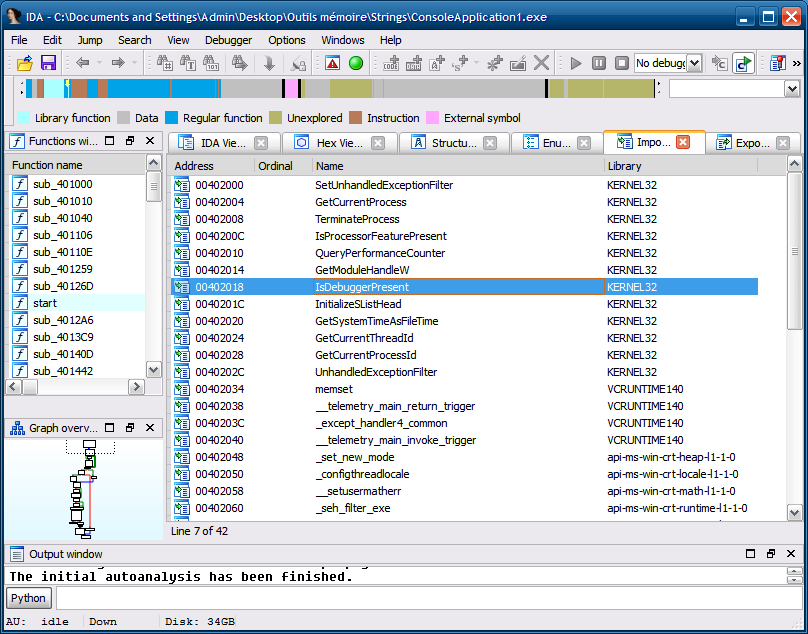
\includegraphics[width=0.8\textwidth]{reverse_engineering/import_table.png}
	\caption{Import table of a program that checks for the presence of a debugger.}
	\label{fig:import_table}
\end{figure}


\paragraph{}
For the IAT to be filled with addresses pointing to another module at runtime, the other module has to specify which functions it is exporting as well as their relative addresses in the module at compile time. This is done with the export table that is also found in the PE header. Once again, they can be listed either by ordinals or by name. If the module decides to export its functions by ordinal, they will have to be imported by ordinal. As such, the verbose identified will be replaced by something more discreet.

\paragraph{}
The other case mentioned above is when dealing with partially compiled code. Because the names declared by the programmers are most of the time kept intact, instead of turning them into addresses, it is possible to go back to a version of the code that is strongly similar to the original one~\cite{eilam2005reversing}. In this situation, the symbolic information cannot be removed. Instead, it can be changed for something less informative. An example would be to replace “isDebuggerPresent” by “fct\_15”.

\subsubsection{Anti Debugging}
\paragraph{}
A debugger is one of the key tools used to carry out reverse engineering, and that makes it a target of choice. With reverse engineers relying on their tool to perform their analysis, confusing the tool would mean confusing the reverse engineer that is sitting at the other side of the tool. This can de achieved in many ways, for example, by exploiting vulnerabilities from the debugger, by changing the behaviour of the program or even by stopping the execution of the program. The book \textit{Practical Malware Analysis}~\cite{sikorski2012practical} proposes many techniques, two of which are presented below.

\paragraph{}
To set breakpoints, debuggers replace the line at which the breakpoint has to be inserted by the INT 3 instructions. One could spawn a thread with the sole purpose of looking for that specific instruction in the sections of the process that contains instructions.

\paragraph{}
Another way of finding INT 3 instructions is to perform checksum on the sections containing instructions. These two protections can be beaten by using hardware breakpoints instead of software ones.

\subsubsection{Confusing Disassemblers}
\paragraph{}
In Section~\ref{disassembler} it has been explained how disassemblers operate to translate machine code into assembly code. It has also been stressed how important a disassembler is to perform reverse engineering for it constitutes the foundation of many other tools such as debuggers and decompilers. As a consequence, it is not uneasy to understand the benefit of embedding anti disassembler protections in one's application. Their goal is to desynchronise the disassembler from the flow of instructions, which will result in an incorrect listing of assembly code.

\paragraph{}
Linear sweep, one of the two methods disassemblers use to decide which part of memory is to be decoded next, works by simply sweeping linearly through the code section. For IA-32 processors, instructions are not all of the same size. Inserting specifically crafted code after a conditional jump can thus desynchronise the disassembler and lead to an incorrect listing. An example can be observed in Listing~\ref{lst:linear_sweep_confused_1} and Listing~\ref{lst:linear_sweep_confused_2}. \\ \\

\noindent\begin{minipage}{.45\textwidth}
	\begin{lstlisting}[caption={The IDA Pro disassembler giving the correct output.}, label={lst:linear_sweep_confused_1}, frame=tlrb, language={[x86masm]Assembler}]
; IDA Pro listing
00401000 jmp short loc_401003
00401002 db   0Ah
00401003 push 0
00401005 push offset Caption
0040100A push offset Text
0040100F push 0
00401011 call MessageBoxA
00401016 push 0
00401018 call ExitProcess
	\end{lstlisting}
\end{minipage}\hfill
\begin{minipage}{.45\textwidth}
	\begin{lstlisting}[caption={The Microsoft WinDbg disassembler giving an incorrect output.}, label={lst:linear_sweep_confused_2}, frame=tlrb, language={[x86masm]Assembler}]
; WinDbg listing
00401000 jmp  0401003
00401002 or   ch,byte ptr [edx]
00401005 push offset Caption
0040100a push offset Text
0040100f push 0
00401011 call MessageBoxA
00401016 push 0
00401018 call ExitProcess
	\end{lstlisting}
\end{minipage}

\paragraph{}
In the example, the two disassemblers correctly translate the first line, an unconditional jump. The second instruction, on the other hand, is not translated correctly by WinDbg. The cause of this problem is that WinDbg uses the linear sweep method, and so mistakes the data for the beginning of the next instruction. Moreover, the third instruction, $push\ 0$, never appears in the listing of WinDbg. This is because the bytes that make this instructions have been consumed to generate the second instruction of the listing. Past that point, WinDbg resynchronises correctly and gives the same result as IDA Pro.

\paragraph{}
As one might have deduced, IDA Pro uses a recursive traversal algorithm, which instead of linearly translating instruction, follows the control flow of the code whenever it encounters a branch or jump instruction. These kind of disassemblers will not fall for the techniques based on the one presented above, but are not exempt of flaws for the cause. Using opaque predicates (see Section~\ref{sec:opaque_predicates}), one can confuse a recursive traversal disassembler with disassembling data.
